%\subsection{Necessity of Training Data}
%The results of these monolingual networks are shown in Figures \ref{figure:mono-per} and \ref{figure:mono-wer}. The same basic trend can be seen for both metrics: there is an elbow in the error rate curves when the training size is somewhere between 2000 and 4000 samples, although it is possible this can be partially explained by other factors, such as higher resource languages having more standardized systems of orthography. The effect of quantity will be explored in more depth in\todo{make this thing}.

%It is not clear, however, how much of this improvement is due to the additional training data and how much could be the result of other factors. One plausible hypothesis is that the data available for the lower resource languages in the set is noisier, and therefore it is more difficult for the model to learn the grapheme-phoneme correspondences for those languages. It could also be possible that higher resource languages, given their higher prestige, are likely to have more 

%\begin{figure}
%\begin{center}
%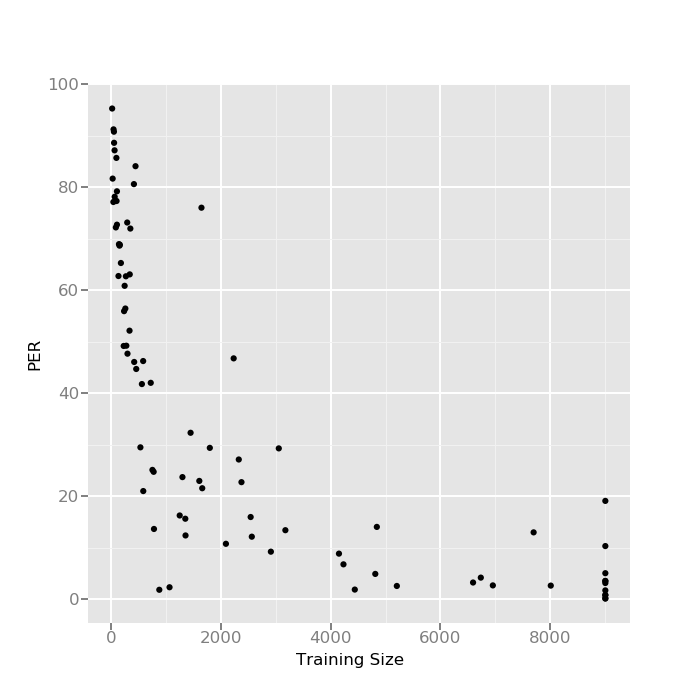
\includegraphics[scale=0.75]{Figures/mono-per}
%\end{center}
%\caption{Phoneme Error Rate by language for the monolingual g2p models.}
%\label{figure:mono-per}
%\end{figure}

%\begin{figure}
%\begin{center}
%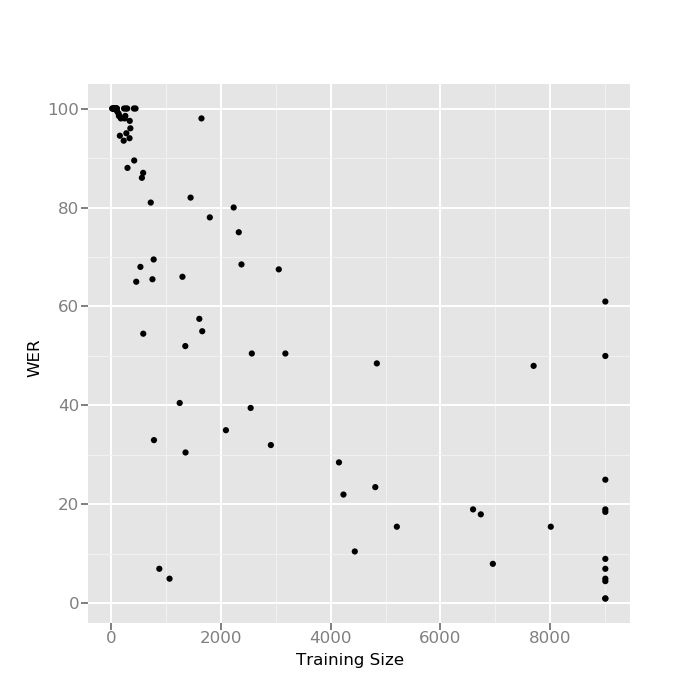
\includegraphics[scale=0.75]{Figures/mono-wer}
%\end{center}
%\caption{Word Error Rate by language for the monolingual g2p models.}
%\label{figure:mono-wer}
%\end{figure}

%Given the clear benefit\todo{this needs to change a little bit, and also I need to get the results} that the multilingually-trained models have on languages with less training data, it would be useful to explore the performance of these models further. Results for the \textsc{LangF-All} and \textsc{LangID-All} models results on the languages used in the previous section are reported below: PER results are shown in Figure \ref{figure:per-by-lang}, WER results are shown in Figure \ref{figure:wer-by-lang}, WER 100 results are shown in Figure \ref{figure:wer100-by-lang}.

%The same basic trend can be seen with all three of these error metrics: among languages with very few training samples (less than about 1000), there is a wide diversity of outcomes: for many of these low-data languages, the models perform very well, and for others very poorly. As the quantity of in-language data increases, results improve. For PER and WER 100 (and to a lesser extent WER), there is an ``elbow'' at around 2000 training samples. Above 2000 samples, performance of the multilingual models is more stable: the worst-performing ones with that much data have PER and WER 100 scores of around 20\%\footnote{The relationship between PER and WER is not consistent across languages because some languages have longer words than others. This is mitigated in WER 100 because the system has so many chances to guess the word correctly.}.

\begin{figure}
\centering
\begin{tabular}{lrrrrrr}
\toprule
{} & \multicolumn{3}{l}{\textsc{LangID-All}} & \multicolumn{3}{l}{\textsc{LangF-All}} \\
{} &        PER & WER & WER 100 &       PER & WER & WER 100 \\
\midrule
bul  &       1.24 &  8.00 &    1.00 &      1.08 &  6.00 &    1.00 \\
deu  &       5.78 & 33.50 &    5.50 &      4.82 & 28.50 &    4.00 \\
eng  &      21.66 & 71.50 &   14.00 &     18.48 & 63.50 &   12.00 \\
epo  &       2.71 &  3.00 &    0.50 &      3.26 &  5.50 &    1.00 \\
fra  &       4.29 & 24.00 &    2.00 &      3.33 & 18.50 &    1.50 \\
hbs  &       0.06 &  0.50 &    0.00 &      0.12 &  1.00 &    0.00 \\
hun  &       1.94 & 11.50 &    0.00 &      1.55 &  9.00 &    0.50 \\
kat  &       0.11 &  1.00 &    0.00 &      0.11 &  1.00 &    0.00 \\
lit  &       1.19 &  9.50 &    0.50 &      1.10 &  8.50 &    1.50 \\
pol  &       3.21 & 18.50 &    1.50 &      3.40 & 20.50 &    1.00 \\
rus  &      11.73 & 56.50 &    4.00 &     11.35 & 54.50 &    4.50 \\
\midrule
Mean &       4.90 & 21.59 &    2.64 &      4.42 & 19.68 &    2.45 \\
\bottomrule
\end{tabular}
\caption{Results of \textsc{LangID-All} and \textsc{LangF-All} models on languages with 9000 training samples and 200 test samples}
\label{figure:big-lang-results}
\end{figure}

%\section{Multilingual Training}
%The clearest innovation of the \textsc{LangID} and \textsc{LangF} models is that they rely on multilingual training. Although I previously showed that this leads to improvements relative to a non-neural baseline, it would additionally be useful to compare the results of the \textsc{LangID} and \textsc{LangF} models against monolingually-trained networks in order to directly test the effect of training on out-of-language data in addition to in-language data.

%\subsection{Data}
%I trained monolingual models for the 84 languages which have a full 200-word test set in \textsc{WikiPronounce}\footnote{It would also have been to train monolingual models for languages with smaller test sets. However, they were excluded because error metrics are more prone to random variation on smaller dataset.}. The number of training samples for these varies from 9, for Medieval Spanish, to 9000, for various high-resource languages. Statistics describing these languages are shown in Table\todo{make} and results of \textsc{LangID-All} and \textsc{LangF-All} on this subset of the test languages is shown in Table\todo{make}.

%\subsection{Training}
%Each model was trained on the same training samples as were present for its language in the training data for \textsc{LangID-All} and \textsc{LangF-All}. The architecture and training conditions are identical to those used for the \textsc{LangID} and \textsc{NoLangID} models, except that the batch size was determined automatically from the training size for each language\todo{how?}. This was necessary because it was impossible to train small datasets with large batch sizes, and larger datasets performed better with larger batch sizes. Because each individual network was monolingual, it was not necessary to add a token or feature identifying the language for any of these models.

%\begin{figure}
%\begin{center}
%\includegraphics[scale=0.7]{Figures/monolingual-per}
%\end{center}
%\caption{Phoneme error rate for monolingually-trained low resource languages}
%\label{figure:lr-per}
%\end{figure}

%\subsection{Results}
%As the results in Figure \ref{figure:lr-per} show, performance was quite poor in the monolingual low-resource case. However, improvement was markedly better when using the multilingually-trained model, as is shown in Figure \ref{figure:multi-improve}.\todo{a table with complete results would be better. So would maybe be training the thing for more languages}

%\begin{figure}
%\begin{center}
%\includegraphics[scale=0.7]{Figures/multi-improve}
%\end{center}
%\caption{Phoneme error rate improvement over for monolingually-trained networks for low resource languages}
%\label{figure:multi-improve}
%\end{figure}
